% This example poster is from Scientific Career Resources
%
% Author:
% Chris Rackauckas <contact@chrisrackauckas.com>
% http://www.chrisrackauckas.com

\documentclass[papersize={48in,36in},dvipsnames,fontmag=.60]{umbcposter}

\usepackage{multicol}
\usepackage{listings}

\usepackage{tikz}
\usepackage{pgfplots}

\usepackage{times}
\usepackage{url}
\usepackage{amsmath}
\definecolor{mitred}{RGB}{163,31,52}
\definecolor{mitdgray}{RGB}{138,139,140}
\definecolor{mitlgray}{RGB}{194,192,191}

% Change the font to Computer Modern Sans Serif
% The default is Times New Roman
\renewcommand{\rmdefault}{cmss}

\begin{document}

\newcommand{\mytitle}{
    \tikz \node[
            fill=white,
            draw=mitred,                   % draw box border
            rounded corners=2ex,
            opacity=0.75,                % background opacity
            text opacity=.9,             % text opacity
            inner sep=0.15\headheight,  % padding around the text
        ] at (0,0) {
            \begin{tabular}{c}
                \Huge ModelingToolkit: A Composable Graph Transformation System for \\
                \Huge Equation-Based Modeling \\
                \huge{Yingbo Ma,
                  Shashi Gowda, Ranjan Anantharaman,
                  Chris Laughman,
                  Viral Shah,
                Chris Rackauckas} \\
                \LARGE{Julia Computing}
            \end{tabular}
    };    % don't forget the semicolon here!
}

\posterinit{
  %grid,
  columns = {3},
  background style = {fill = mitlgray},
  title = {\mytitle},
  %left logo = {
\includegraphics[height=0.75\headheight]{figures/pumas.pdf}},
  %right logo = {
\includegraphics[height=0.5\headheight]{figures/MIT-logo-with-spelling-print-black-red-design1}},
  box/border style= {draw = black, line width = 1pt},
  box/header style = {top color = mitred, bottom color = mitred, middle color = mitred, fill opacity = .9},
  box/header font color = {white},
  box/header font = {\large\rm},
  box/body style = {fill = white, fill opacity=.85},
  head height = {0.15\textheight},
  box/all rounded
}

\boxit{col = 0, at top, name=problem}{ModelingToolkit Overview}{
  ModelingToolkit is a general-purpose Computer Algebra System (CAS) in the
  Julia programming language, as the core expression representation for
  ModelingToolkit, which allows for efficient application of expression
  rewriting.
  \vspace{13pt}

  The modeling domain of MTK covers the span of:
  \begin{itemize}
    \item Ordinary differential(-algebraic) equations (\texttt{ ODESystem })
    \item Stochastic differential(-algebraic) equations (\texttt{ SDESystem })
    \item Partial differential equations (\texttt{ PDESystem })
    \item Nonlinear solve equations (\texttt{ NonlinearSystem })
    \item Optimization problems (\texttt{ OptimizationSystem })
    \item Continuous-Time Markov Chains (\texttt{ JumpSystem })
    \item Nonlinear Optimal Control (\texttt{ ControlSystem })
  \end{itemize}
  \vspace{13pt}

  For example, the following code builds and solves the classic Lorenz '63
  system:
  \begin{center}
    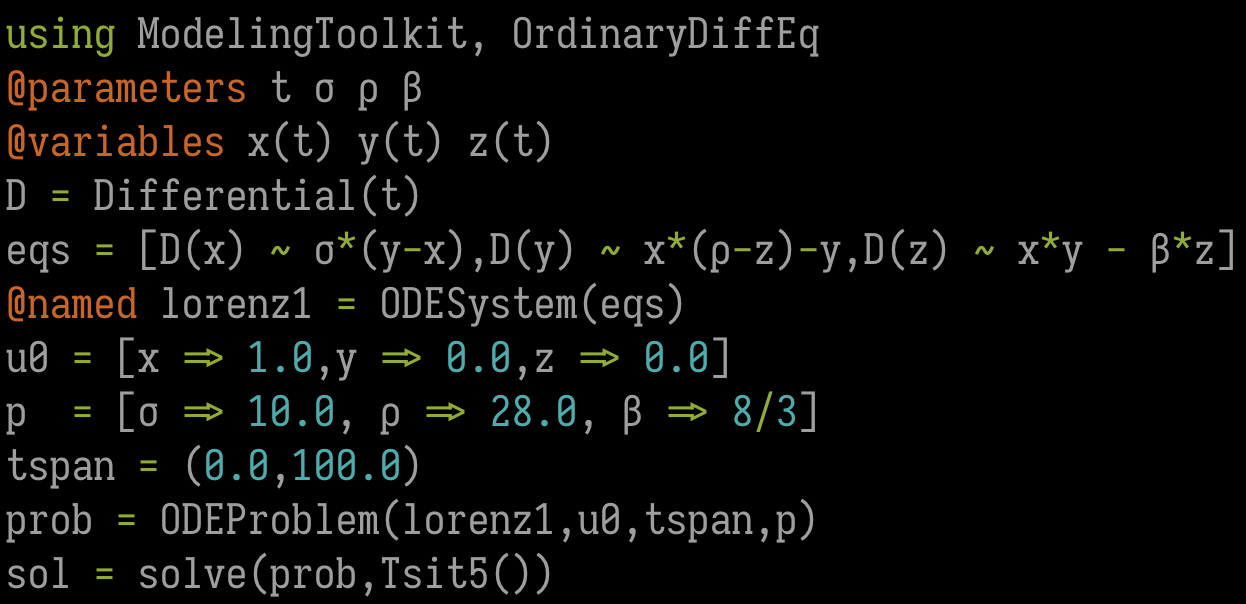
\includegraphics[width=220px]{figures/lorenz.png}
  \end{center}
  As an acausal modeling system, one can also arbitrarily compose system
  components and generate differential-algebraic equations by placing algebraic
  relations between the variables. The following extends the previous example to
  show how to connect a second instance of the Lorenz \texttt{ODESystem} to the
  first, with an algebraic variable defined implicitly by their connection:
  \vspace{9pt}
  \begin{center}
    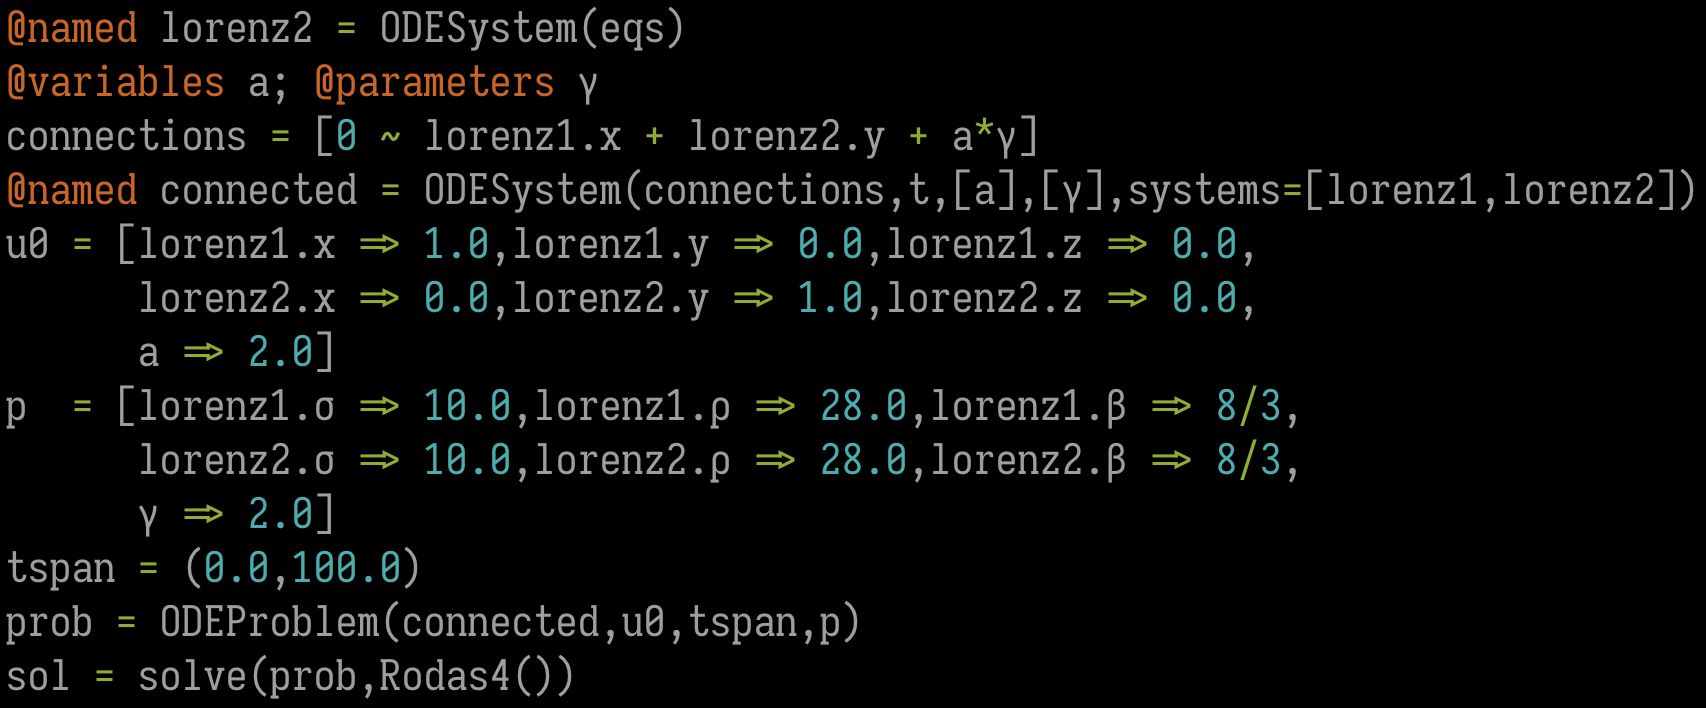
\includegraphics[width=220px]{figures/lorenz2.png}
  \end{center}
  \vspace{11pt}
}

\boxit{at top, col = 1, name=box3}{Index Reduction of Numerical Code}{
  Cartesian pendulum (index 3 system):
  It has 5 state variables, $x$, $y$, the velocities $v_x$ and $v_y$,
  and $T$, with parameters $g$ for the acceleration due to gravity and the fixed
  length of the pendulum $L$.
  \begin{align}
    x^\prime &= v_x\\
    v_x^\prime &= Tx\\
    y^\prime &= v_y\\
    v_y^\prime &= Ty - g\\
    0 &= x^2 + y^2 - L^2
  \end{align}
  Numerical code would be
  \begin{center}
    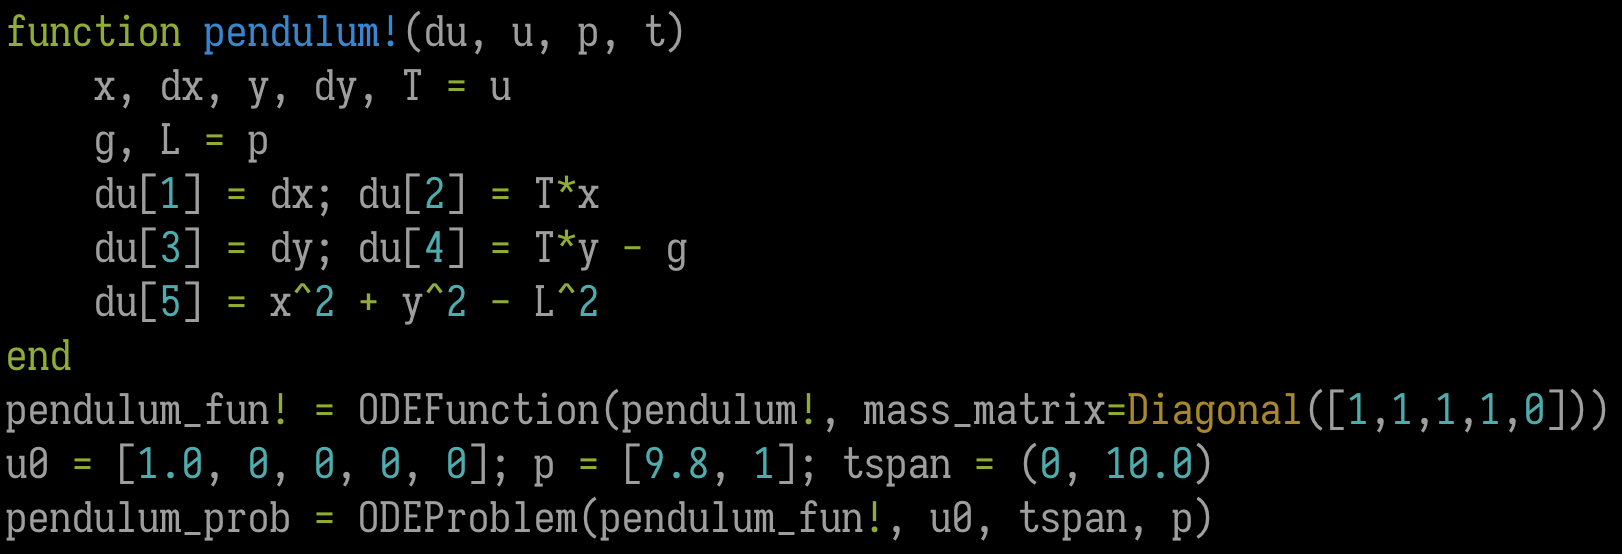
\includegraphics[width=220px]{figures/code3.png}
  \end{center}

  We can reduce the index of numerical code by symbolically tracing into the
  system.
  \begin{center}
    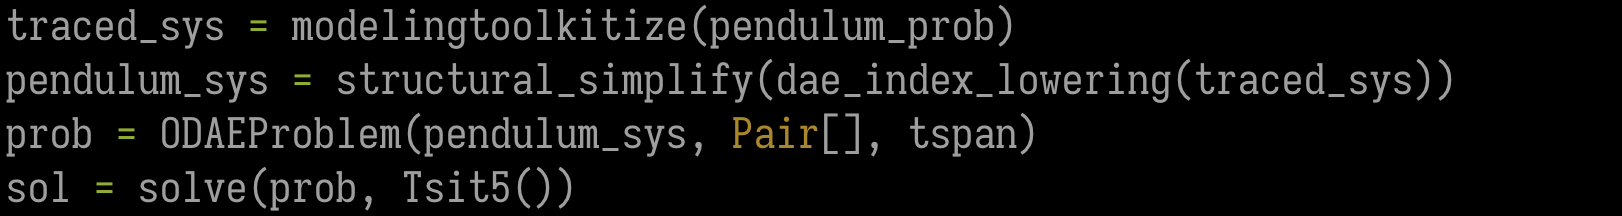
\includegraphics[width=220px]{figures/code4.png}
  \end{center}
  From the traced system, ModelingToolkit automatically generates the index 1
  system
  \begin{align}
    x^\prime =& v_x \\
    v_x^\prime =& x T \\
    y^\prime =& v_y \\
    v_y^\prime =& y T - g \\
    0 =& 2 \left(v_x^{2} + v_y^{2} + y ( y T - g ) + T x^2 \right)
  \end{align}
  \begin{center}
    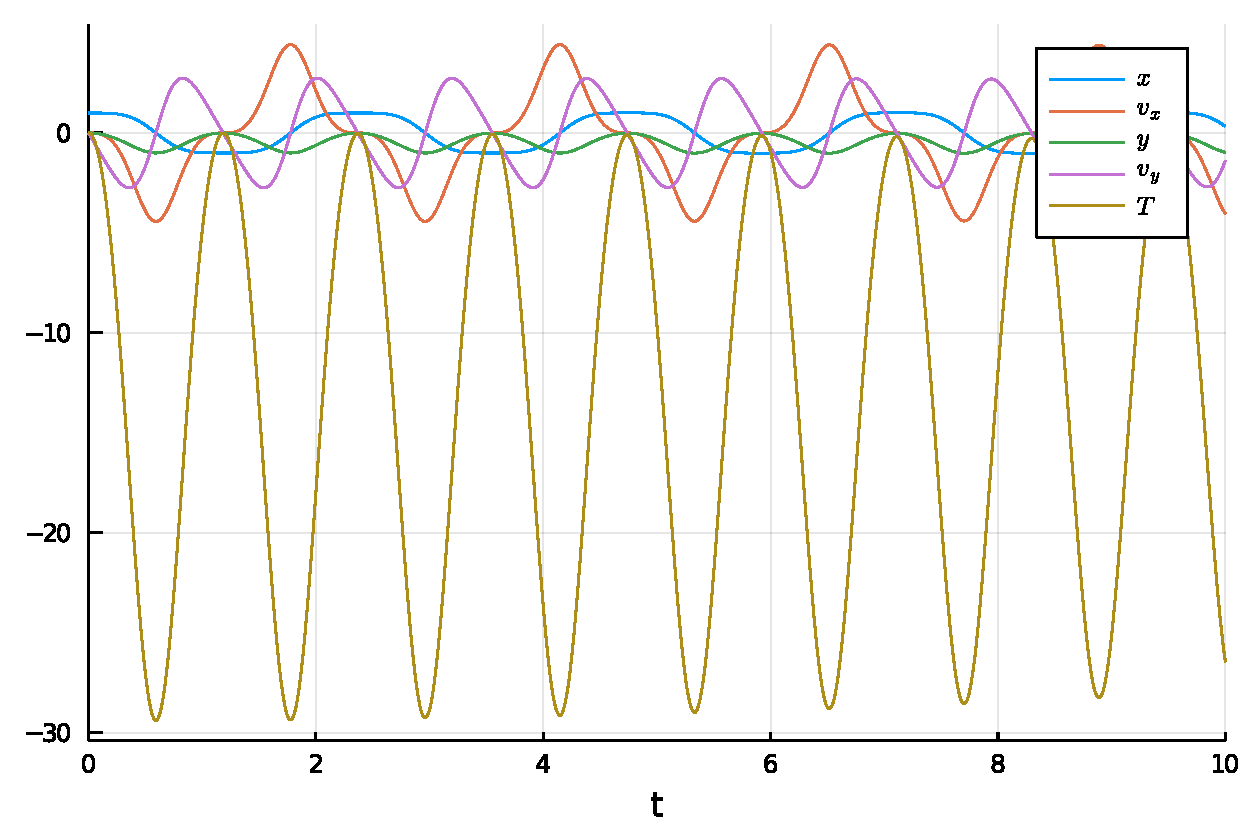
\includegraphics[width=200px]{figures/pend.pdf}
  \end{center}
}

\boxit{at top,col = 2, name=events}{Extracting Parallelism from Structural Simplification}{
  Using the block lower triangular sorting, ModelingToolkit is able to
  parallelize nonlinear system solving.

  The incidence matrix of 50 independent RC circuits whose resistance is a
  non-linear function of the ambient temperature, and that of a model of an HVAC
  system are shown. A non-zero $(i,j)$-th entry means $j$-th variable appears in
  $i$-th equation. Each connected component in the subfigures in the second and
  third column imply a single call to solver to obtain the values of the
  algebraic variables in that component.  ModelingToolkit is able to detect
  independence between components and spawn these calls in parallel. Note that
  we only show algebraic equations and algebraic variables in the Block Lower
  Triangular (BLT)-sorted spy plots, because only the algebraic part of the
  system has a non-trivial dependency structure that we need to analyze for
  parallel executions.
  \begin{center}
    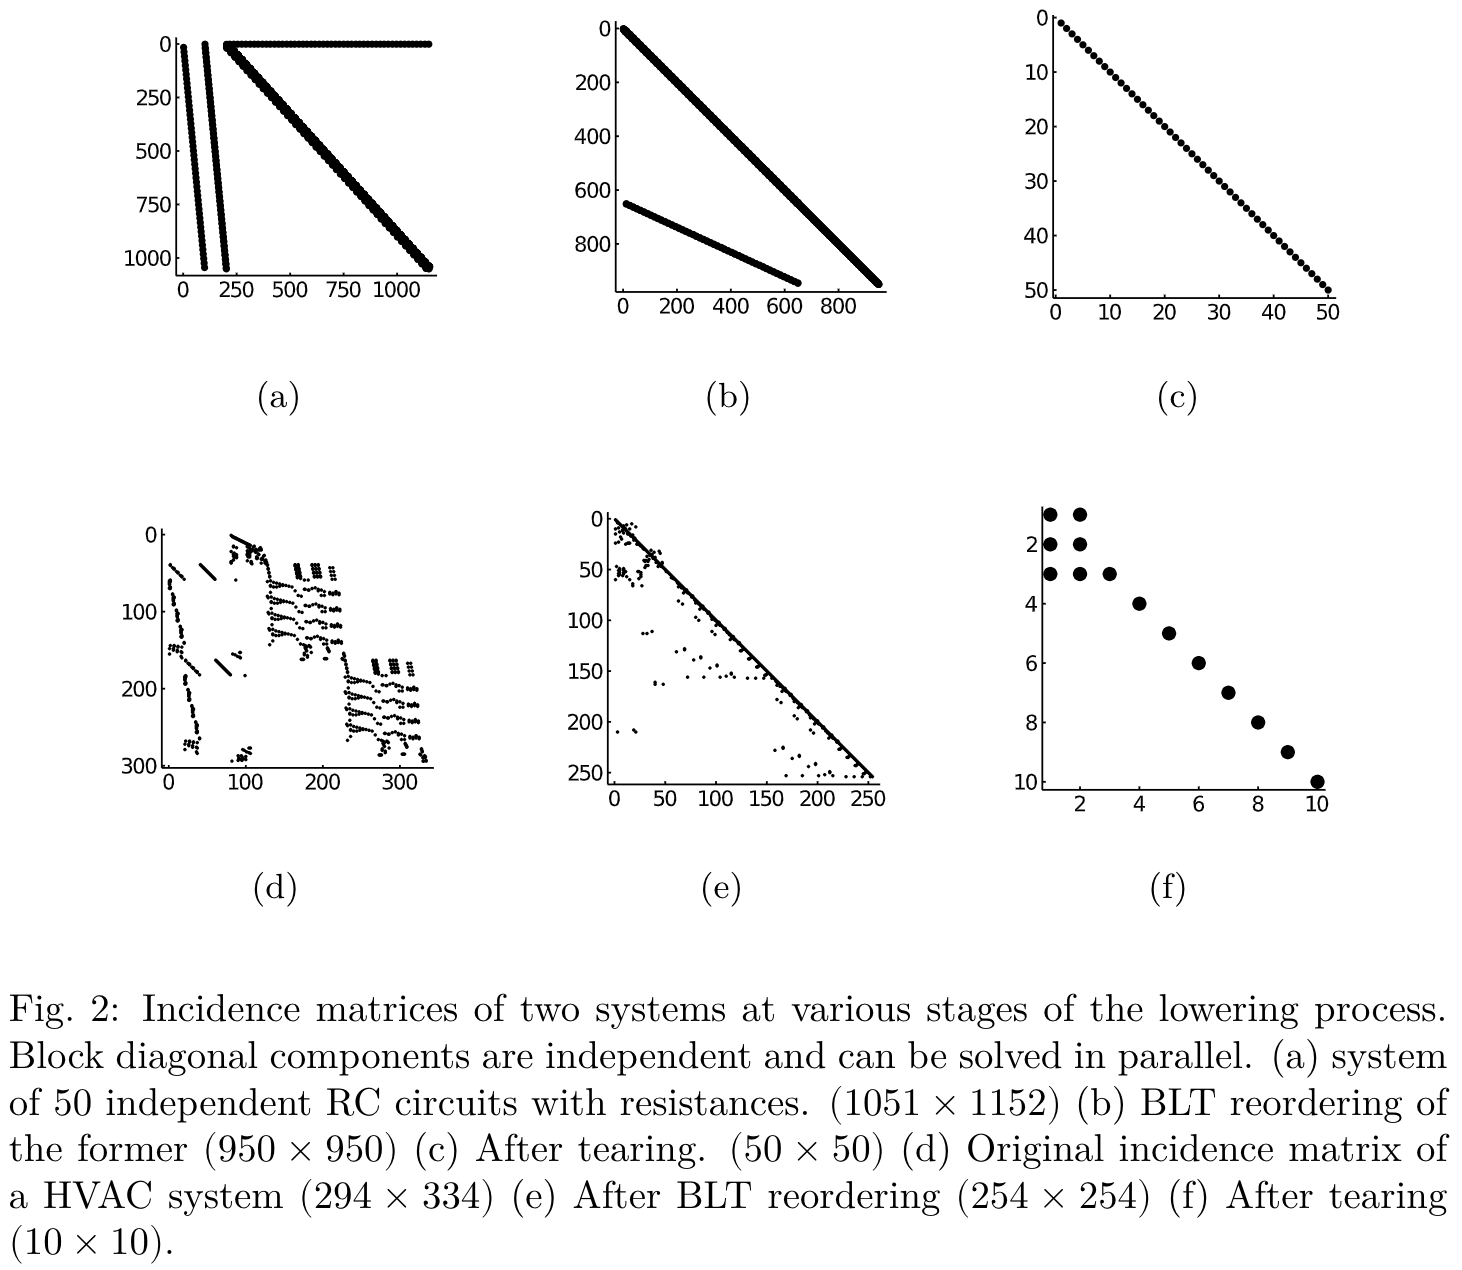
\includegraphics[width=200px]{figures/par.png}
  \end{center}

}

\boxit{below of = events,col = 2, name=conc}{Conclusion}{
  While discrete graph-based algorithms have been added before to equation-based
  modeling environments to improve stability and performance, ModelingToolkit is
  the first to embed such a modeling environment directly into a high
  performance host language and allow for composable transformations to be
  constructed using a CAS. In a sense, this extends the abstract interpretation
  techniques of automatic differentiation to directly perform arbitrary symbolic
  transformations on a user's code for alternative mathematical purposes.
  \vspace{10pt}
}

\boxit{below of = conc,col = 2, name=ack}{Acknowledgments}{
  The information, data, or work presented herein was funded in part by the
  Advanced Research Projects Agency-Energy (ARPA-E), U.S. Department of Energy,
  under Award Number DE-AR0001222 and NSF grants OAC-1835443 and IIP-1938400. We
  additionally thank Simon Frost of Microsoft Research Studies in Pandemic
  Preparedness for helping fund this work. The views and opinions of authors
  expressed herein do not necessarily state or reflect those of the United States
  Government or any agency thereof.
  \vspace{9.5pt}
}

\end{document}
